\documentclass{ctexart}

\usepackage{graphicx}
\usepackage{hyperref}
\usepackage{amssymb}
\usepackage{amsmath}

\DeclareMathOperator*{\argmax}{arg\,max}
\DeclareMathOperator*{\argmin}{arg\,min}

\title{基于可微分渲染的人脸3D重建}
\author{胡玮文}

\begin{document}

\maketitle

\tableofcontents

\listoffigures

\section{绪论}

\section{相关研究综述}

\section{适应未知背景的无偏可微分渲染技术}

\subsection{问题定义}

可微分渲染旨在从参数化的3D模型,如三角形面片,纹理贴图等,渲染得到2D图片,同时计算该渲染结果关于其输入参数的梯度,以期利用基于梯度的方法优化输入参数,从而改善渲染效果。

然而现有方法存在一些不足:
\begin{enumerate}
    \item 现有可微分渲染技术大多是对整张图片估计梯度,即不区分前景和背景部分。然而,在基于自然环境照片的人脸重建任务中,我们通常只有前景(即人脸)的3D模型,而没有背景的模型。若只使用人脸模型拟合整张图片则无法得到合理的结果,在缺乏关于照片背景的先验知识时也难以对照片背景进行显式建模。
    \item 现有的一些梯度估计方法是有偏的,即该梯度无法指引模型收敛到局部最优点。另一些无偏的方法则有一些其他缺陷,有些计算量大、梯度噪声大,有些会在渲染结果中引入少量模糊等。这些缺陷会导致模型收敛的速度和精度下降,甚至无法收敛到较合理的解。
\end{enumerate}

\subsection{本文方法}

\paragraph{收缩\&扩展约束}(创新点)

\paragraph{基于纹理坐标的无偏几何梯度估计}(预估创新点,尚未实验)

\subsection{实验结果}

\subsection{讨论}

\section{基于可微分渲染的人脸3D重建}

\subsection{基于单张自然环境照片的人脸重建}

\subsection{基于多视角实验室照片的人脸重建}

\subsubsection{问题定义}

输入多个相机在(几乎)同一时刻拍摄的肖像照片。相机的参数和环境光照可以提前标定。本文的目标是静态模型重建,因此无须考虑采集连续动态图像的问题。通过以很小的间隔(数毫秒)触发多盏闪光灯,也能在单次采集中获得不同照明条件的数据。

输出被拍摄对象尽可能精确的3D模型,并能支持任意视角,任意光照条件下重新渲染。

本文的贡献主要在于采集系统的搭建方案,以及结合我们特定情况的算法复现和改进。

\subsubsection{相机固定}

铝型材支架设计

\subsubsection{被动相机同步}
\label{sec:passive_sync}

该装置无须独立供电。它能以很高的精度同时触发多台单反相机的对焦和快门,从而实现人脸多视角数据的捕获。

\paragraph{单反相机快门触发原理}

\paragraph{同步装置硬件设计}

\paragraph{同步精度测试}

\subsubsection{多相机内外参联合标定}

为了建立三维物体与二维照片之间的准确对应关系,需要对相机的内参和外参进行标定。
即准确测量采集过程中用到的每一台相机的内参和外参。
其中,内参包括相机的焦距、光心坐标、畸变参数等,
外参则包括不同相机之间的相对位置和姿态。

本文选用的相机模型是针孔相机模型,这也是在实验中采用的相机所遵循的模型。
由于本实验中相机畸变较小,简单起见,本文选用了OpenCV中默认的径向和切向相机畸变模型\cite{?}。
更正式地,假设共有N个相机,对于第$i$个相机($i=1,2,\cdots,N$),
内参标定的目标是求解该相机的
焦距$f_x^{(i)},f_y^{(i)}$、
光心坐标$c_x^{(i)},c_y^{(i)}$、
畸变参数$k_1^{(i)},k_2^{(i)},k_3^{(i)},p_1^{(i)},p_2^{(i)}$;
外参标定的目标则是求解该相机在世界坐标系下的
位置$\mathbf{t}^{(i)}=\left(x^{(i)},y^{(i)},z^{(i)}\right)$
和姿态$\mathbf{r}^{(i)}$。
其中$\mathbf{r}\in \mathbb{R}^3$为表示旋转的罗德里格斯向量\cite{?}。
世界坐标系的选取是任意的,因此在相机标定阶段,不失一般性地,我们选择第一个相机作为世界坐标系。
即令$\mathbf{t}^{(1)}=\mathbf{0}$,$\mathbf{r}^{(1)}=\mathbf{0}$。
综上,在标定过程中共需要求解$N\times 15 - 6$个参数,记为$\delta$。

在该模型下,对于任意在世界坐标系下的点$\mathbf{X}=\left[X,Y,Z\right]^\mathsf{T}$,其在第$i$个相机的成像平面的投影点$\mathbf{x}^{(i)}$可以通过如下方式计算(简洁起见,此后省略上标$(i)$):
首先,将$\mathbf{X}$从世界坐标系转换到第$i$个相机的坐标系,即
\begin{align}
    \theta &= \left\|r\right\|_2 \\
    \hat{\mathbf{r}} &= \mathbf{r}/ \theta \\
    \mathbf{R} &= \cos(\theta) I + (1- \cos{\theta} ) \hat{\mathbf{r}} \hat{\mathbf{r}}^\mathsf{T} + \sin(\theta) \begin{bmatrix}
         0   & -\hat{\mathbf{r}}_z & \hat{\mathbf{r}}_y \\
         \hat{\mathbf{r}}_z & 0    & -\hat{\mathbf{r}}_x \\
        -\hat{\mathbf{r}}_y &  \hat{\mathbf{r}}_x & 0
    \end{bmatrix} \\
    \mathbf{X}' &= \mathbf{R} \mathbf{X} + \mathbf{t}\text{,}
\end{align}
然后,将$\mathbf{X}'$投影到第$i$个相机的成像平面,即
\begin{equation}
    \mathbf{x}'' = \begin{bmatrix}
        \mathbf{X}'_x / \mathbf{X}'_z \\
        \mathbf{X}'_y / \mathbf{X}'_z
    \end{bmatrix}\text{,}
\end{equation}
对$\mathbf{x}''$应用镜头畸变,即
\begin{equation}
    \mathbf{x}' = \left(1 + k_1 r^2 + k_2 r^4 + k_3 r^6\right) \mathbf{x}'' + \begin{bmatrix}
        2 p_1 \mathbf{x}''_x \mathbf{x}''_y + p_2 \left(r^2 + 2 (\mathbf{x}''_x)^2\right) \\
        p_1 \left(r^2 + 2 (\mathbf{x}''_y)^2\right) + 2 p_2 \mathbf{x}''_x \mathbf{x}''_y
    \end{bmatrix}\text{,}
\end{equation}
其中$r = \left\|\mathbf{x}''\right\|_2$。最后,将$\mathbf{x}'$映射到以左上角为原点的像素坐标系,即
\begin{equation}
    \mathbf{x} = \begin{bmatrix}f_x & 0 \\ 0 & f_y \end{bmatrix} \mathbf{x}' + \begin{bmatrix}c_x \\ c_y \end{bmatrix}\text{。}
\end{equation}
以上过程可称为相机投影,记为$\pi(\delta_i, \cdot)$。

为了解算上述模型中的参数,通常需要使用待标定的相机对一类特殊的物体进行拍摄,称为标定物体。
它们的特点是通常有一些在照片中容易被计算机视觉算法识别的特征点,且这些点容易在不同相机拍摄的照片间进行匹配。
这类物体通常为标定板,即印有棋盘格、二维码、圆形或者其他易于识别的图案的硬质平面板子。
也有一些方法\cite{colmap}使用SIFT等特征点算法来自动从任意被拍摄物体上提取和匹配特征点。但这种方法匹配成功率稍低,且忽略了物体反射光线的各向异性,因此可能会带来一些误差。

\begin{figure}
    \centering
    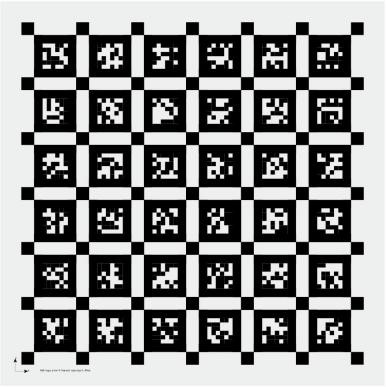
\includegraphics[width=0.5\textwidth]{figures/april_board}
    \caption{April Board上印制的二维码和棋盘格图案}
    \label{fig:april_board}
\end{figure}

本文中使用的标定物体为April Board,即印有二维码和棋盘格组成的图案的标定板,如图\ref{fig:april_board}所示。
该标定板的尺寸为$800 \times 800$毫米,每个二维码的边长为$88$毫米。
该图案中棋盘格的十字角点可由算法精确完成亚像素级定位,而密集的二维码则便于在不同相片中便捷地匹配角点。
其采用了玻璃基板,以保证标定板的刚性和平整度;
同时采用了氧化铝表面,使标定板表面无明显镜面反射光斑,确保标定板在不同光照条件下的可靠性。

在拍摄标定物体时,首先将相机固定到支架上,将任意物体摆放至预计人脸的位置作为调节的参照,并完整相机角度调节和对焦操作。
将相机切换至手动对焦模式,以防止其内参意外发生变化。
然后,撤走参照物,将标定板放在该位置,使用前述(第\ref{sec:passive_sync}节)被动相机同步装置同时触发所有相机进行拍摄。转动标定板,重复触发20-30次快门。

\paragraph{相机标定原理}本文中的相机标定算法接收照片中的特征点坐标作为输入,求解上述相机模型中的参数$\delta$。
正式地,假设共触发了$M$次快门,标定板中共有$K=144$个角点,算法的输入包括第$i$个相机的第$j$次触发快门拍摄中的第$k$个角点($j = 1,2,\cdots,M$、$k = 1,2,\cdots,K$)在像素坐标系中的坐标$o_{i,j,k}\in \mathbb{R}^2$;
以及角点在标定板坐标系中的坐标$w_k\in \mathbb{R}^3$。
由于每次触发快门时标定板都由人工转动,因此其在世界坐标系中的位置也是未知的,故将第$j$次快门时标定板坐标系到世界坐标系的刚体变换$T_{j}(\cdot)\in SE(3)$也做为未知量。
则本文中的相机标定问题可以表示为以下最小二乘优化问题:
\begin{equation}
    \argmin_{\delta,T} \sum_{i=1}^N \sum_{j=1}^M \sum_{k=1}^K \left\| o_{i,j,k} - \pi\left(\delta_i, T_j(w_k)\right) \right\|^2
\end{equation}

\paragraph{二维码识别}尺度、对比度无关的二维码定位算法(创新点?不知道够不够格)

\paragraph{角点精确定位}二维多项式函数的拟合与鞍点查找

\paragraph{多相机内参标定与外参传递}

\paragraph{集束调整}

\paragraph{标定结果和误差分析}

\subsubsection{主动相机/闪光灯同步}

主动相机同步装置有单片机等实时控制系统控制,能独立控制每台相机、闪光灯触发延迟,最多24个通道。可用于快速抓拍不同闪光灯照明下的照片

\paragraph{主动同步装置硬件设计}

\paragraph{主动同步装置软件设计}

\paragraph{滚动快门原理}

\paragraph{闪光灯触发延迟快速标定方法}

\subsubsection{基于反射球的光源标定和HDRI合成}

\subsubsection{基于可微分渲染的3D重建}

\paragraph{3D模型初始化}

\paragraph{基于物理的可微分逆渲染}

\section{结论与展望}

\section*{参考文献}

\section*{致谢}

\end{document}
